\begingroup
\captionsetup{font=footnotesize,skip=3pt,hypcap=false}
\setlength{\abovecaptionskip}{3pt}
\setlength{\belowcaptionskip}{0pt}

\subsection{Detailed directed OD rankings}
The following compact pages show the ten leading directed OD pairs by trip volume and by aggregate passenger spending for each service and month. The original map images are unchanged; only their placement in the supplement is condensed.

\begin{center}
\centering
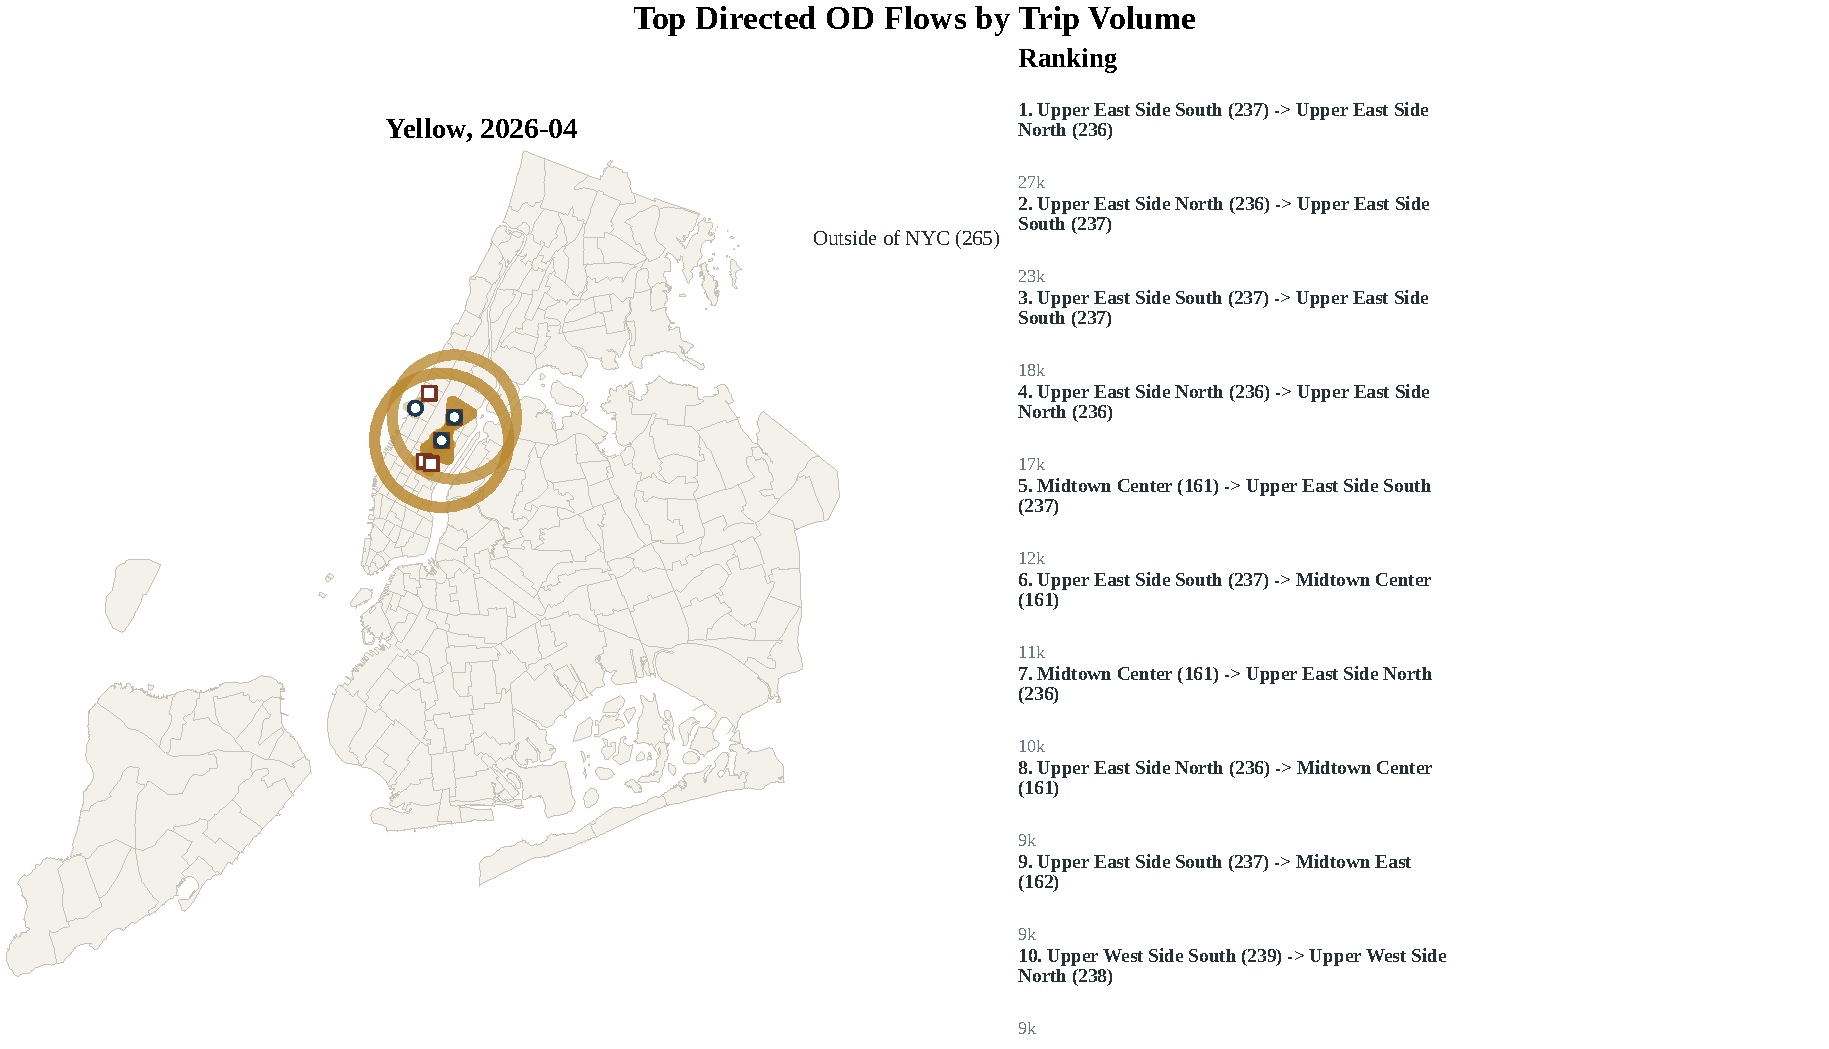
\includegraphics[height=.265\textheight,width=.98\linewidth,keepaspectratio]{04_Results/report_figures/appendix/task2_od_volume_2026-04_yellow.pdf}\par\vspace{0.2em}
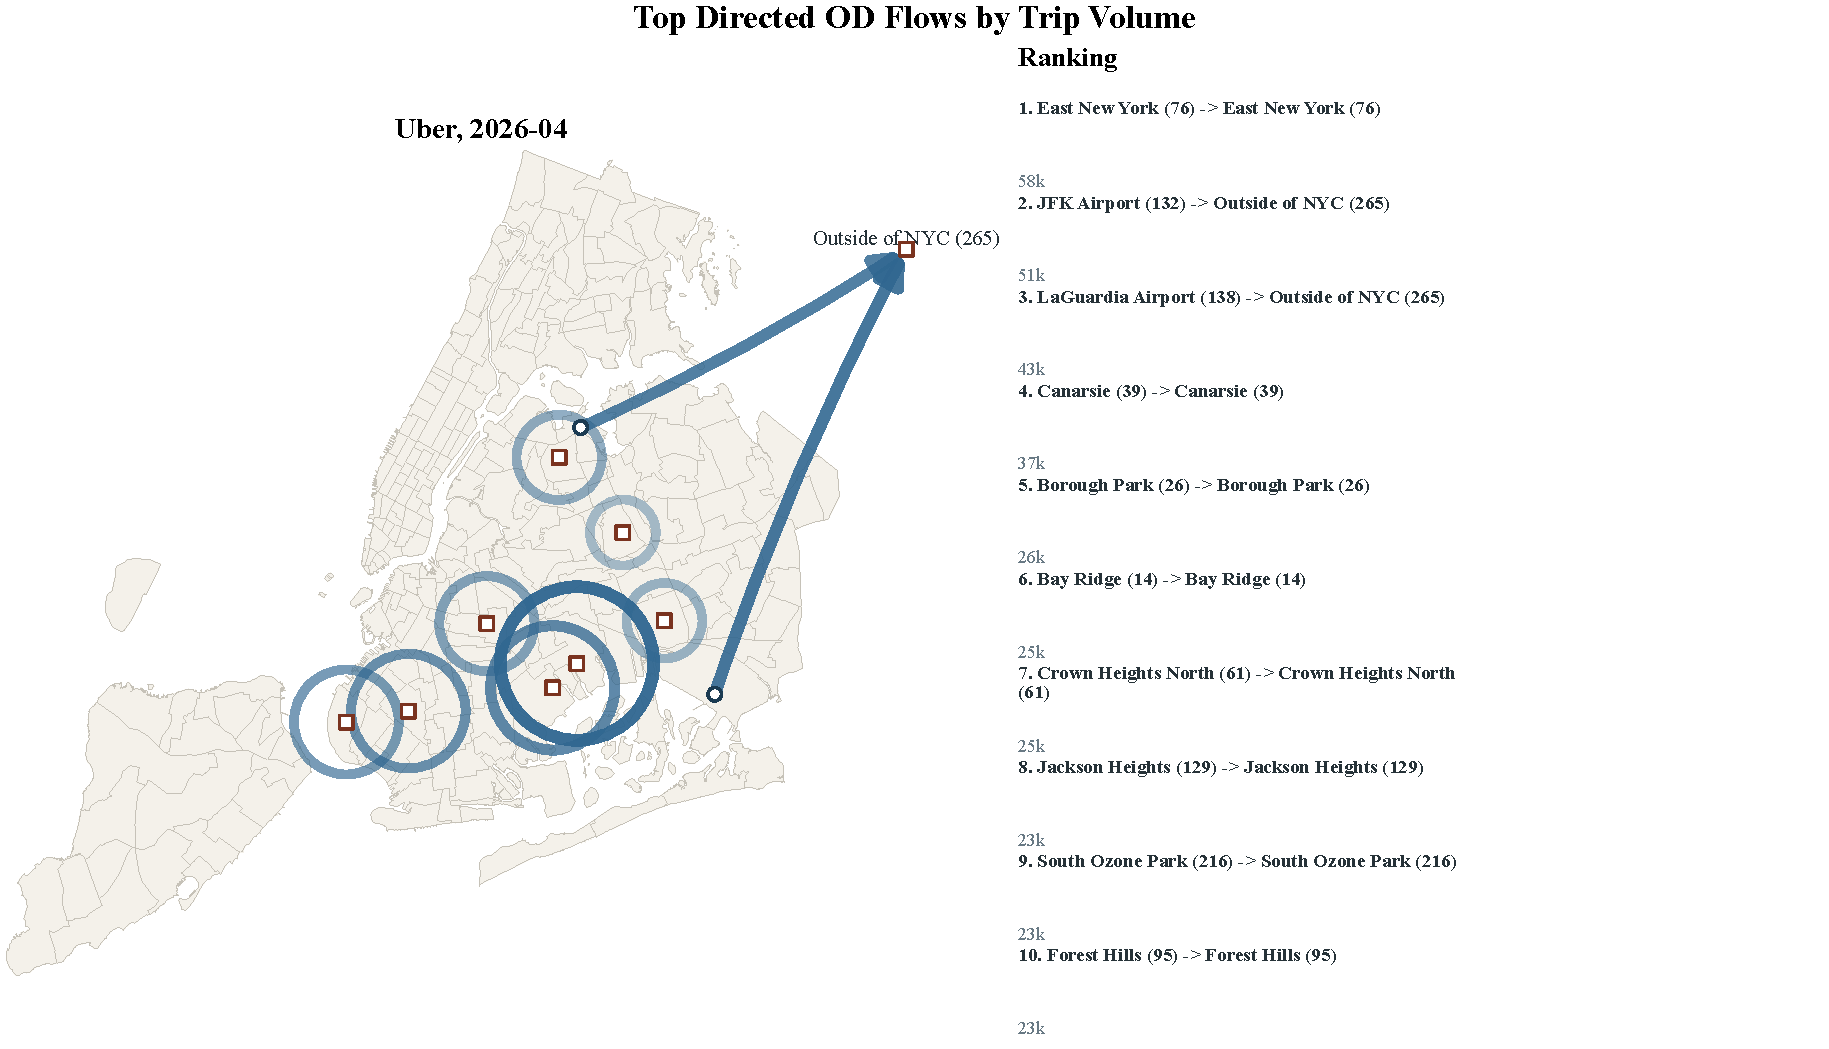
\includegraphics[height=.265\textheight,width=.98\linewidth,keepaspectratio]{04_Results/report_figures/appendix/task2_od_volume_2026-04_uber.pdf}\par\vspace{0.2em}
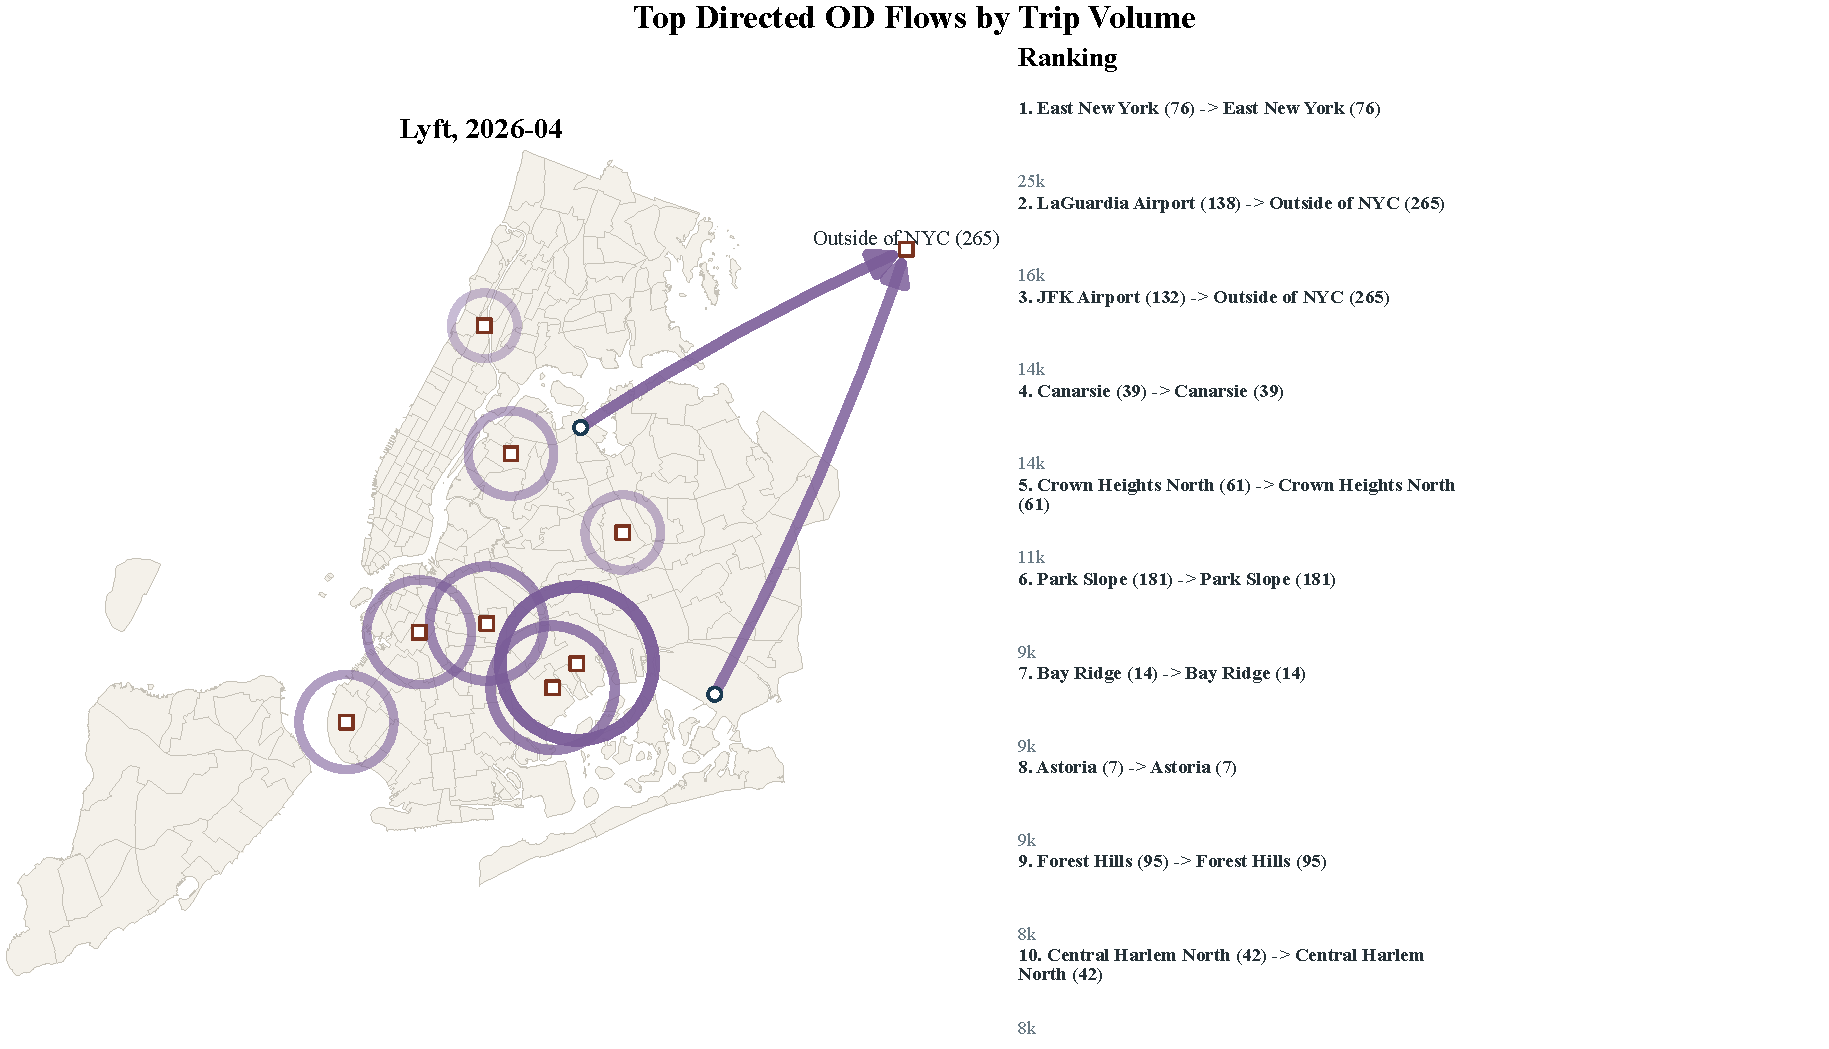
\includegraphics[height=.265\textheight,width=.98\linewidth,keepaspectratio]{04_Results/report_figures/appendix/task2_od_volume_2026-04_lyft.pdf}
\captionof{figure}{Top ten OD flows by trip volume, 2026-04. Panels from top to bottom: Yellow Taxi, Uber, and Lyft.}
\end{center}
\clearpage

\begin{center}
\centering
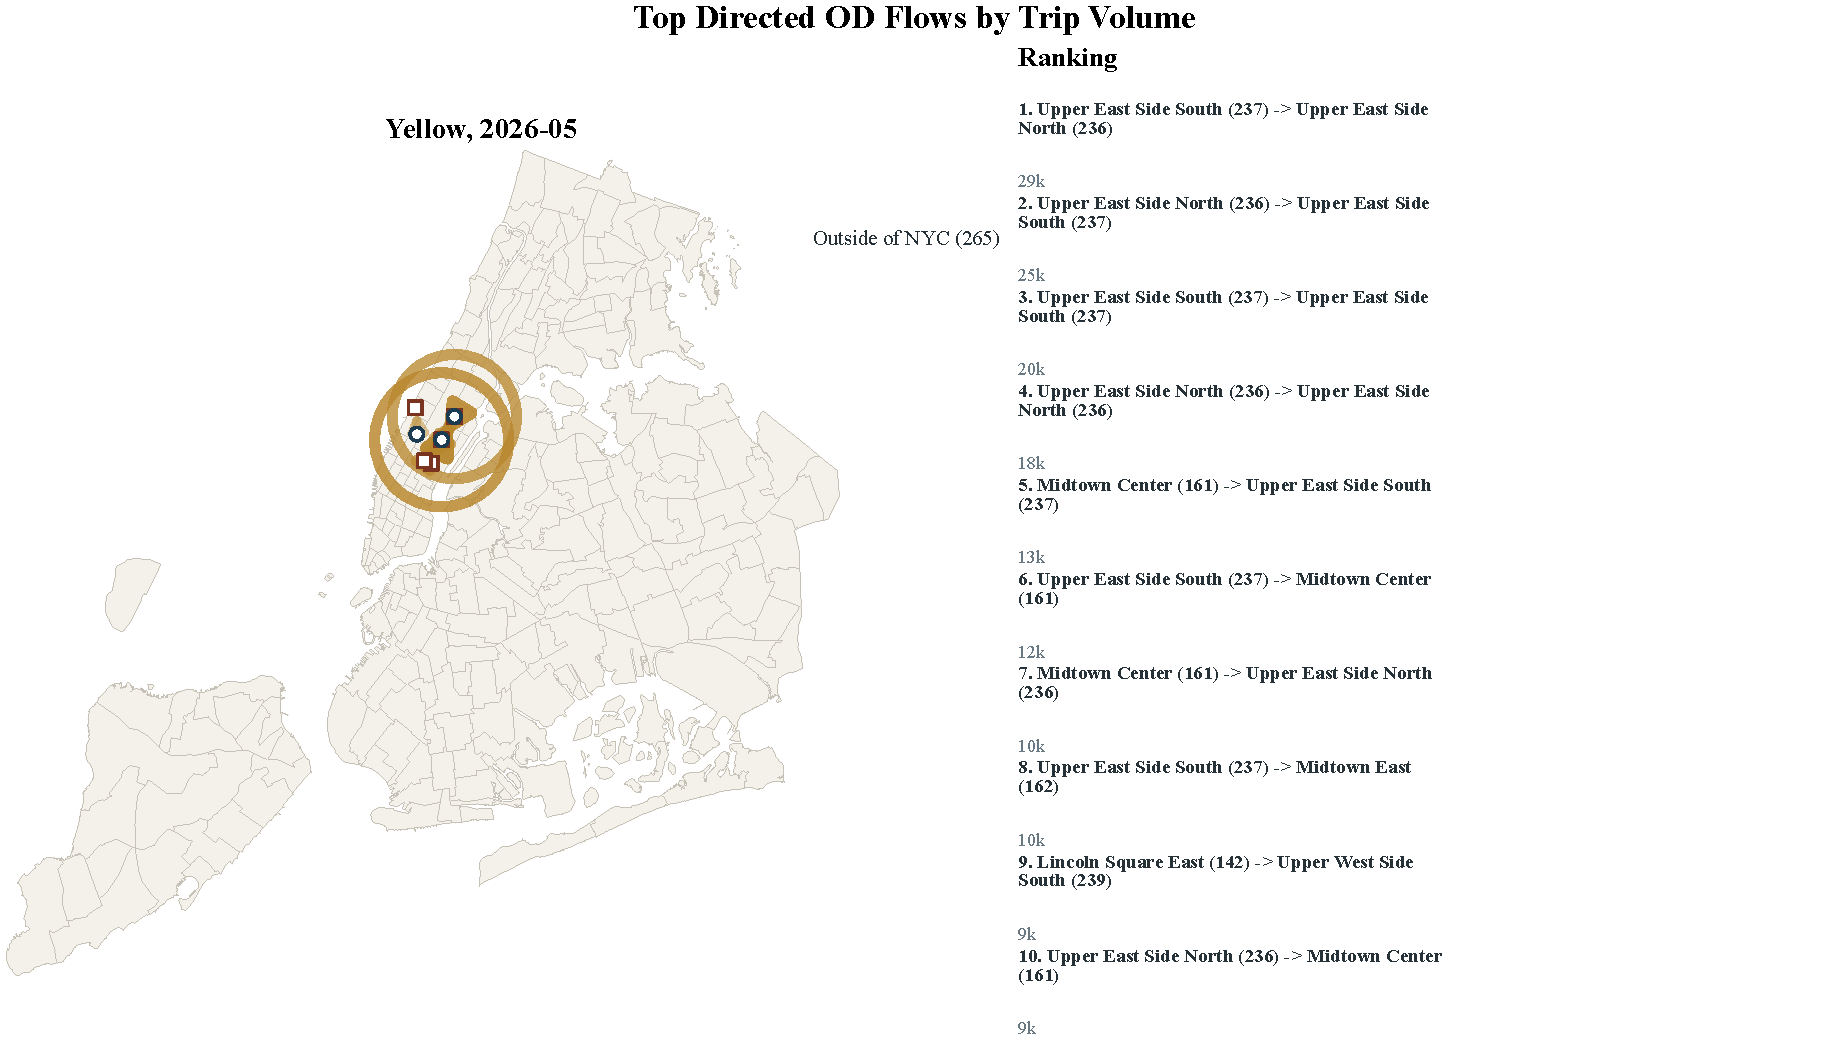
\includegraphics[height=.265\textheight,width=.98\linewidth,keepaspectratio]{04_Results/report_figures/appendix/task2_od_volume_2026-05_yellow.pdf}\par\vspace{0.2em}
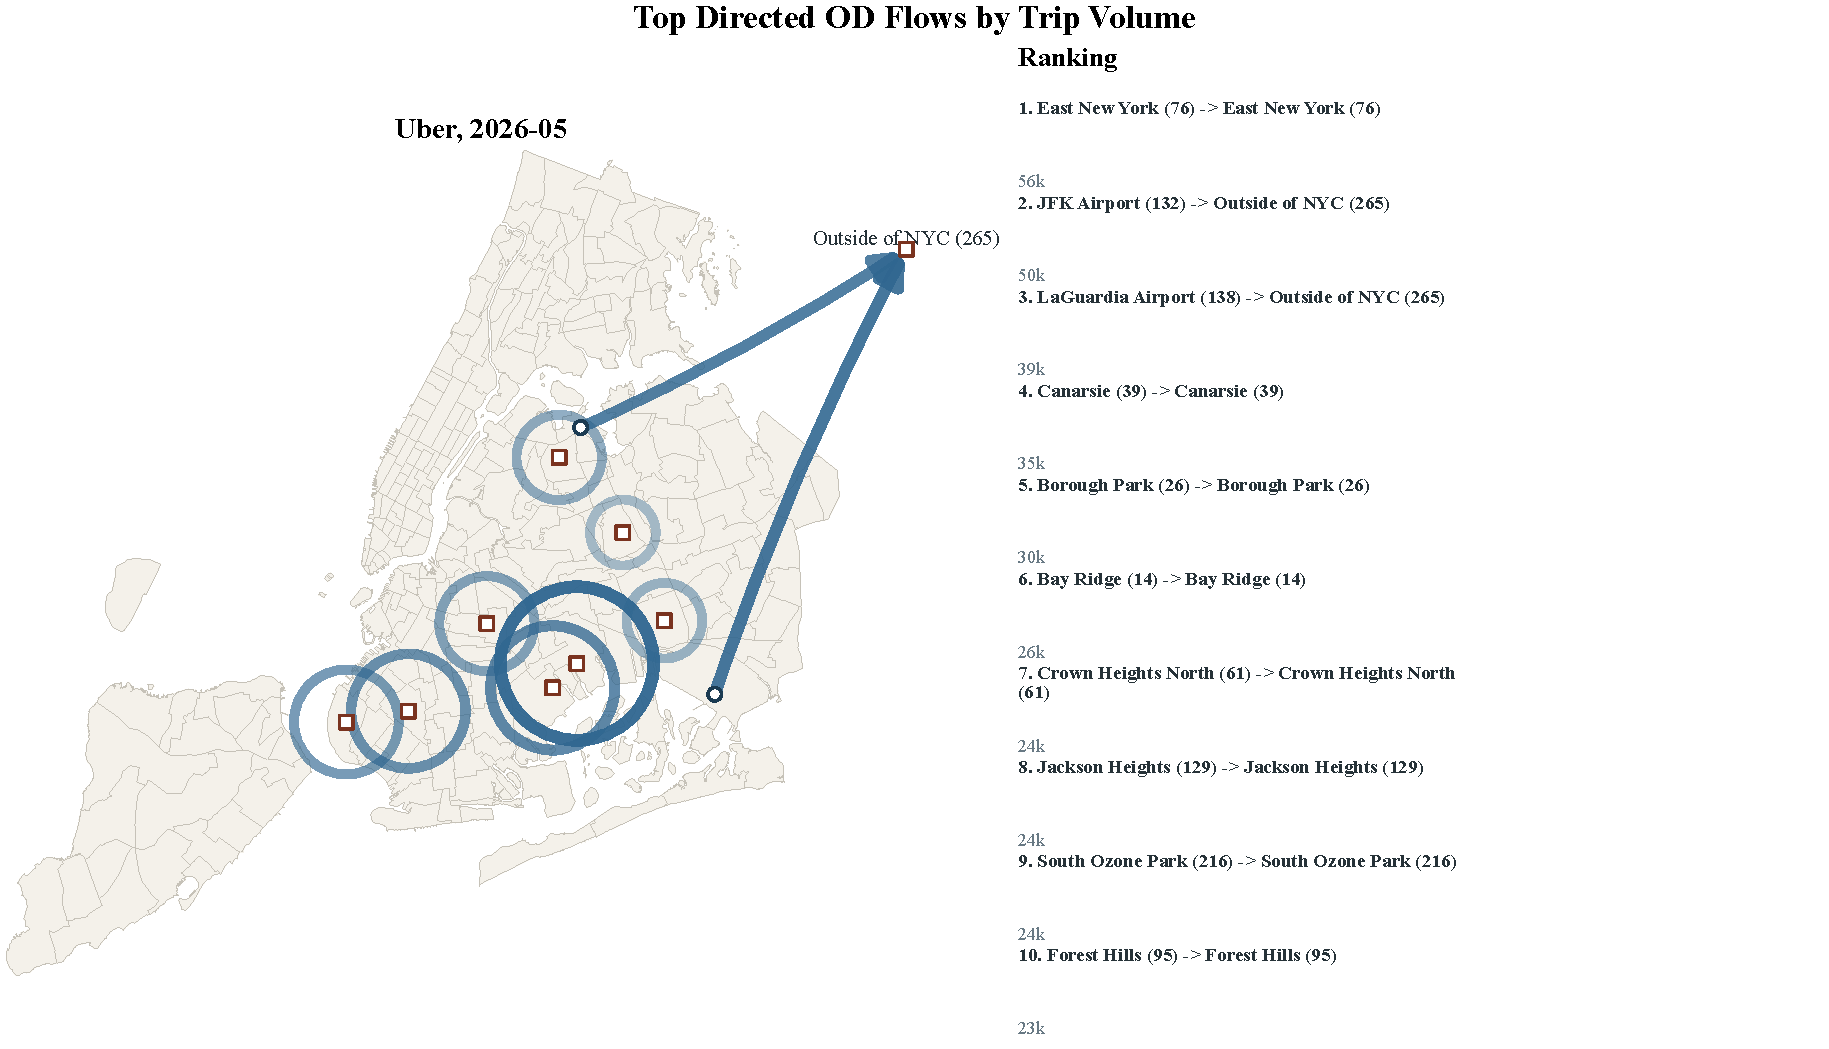
\includegraphics[height=.265\textheight,width=.98\linewidth,keepaspectratio]{04_Results/report_figures/appendix/task2_od_volume_2026-05_uber.pdf}\par\vspace{0.2em}
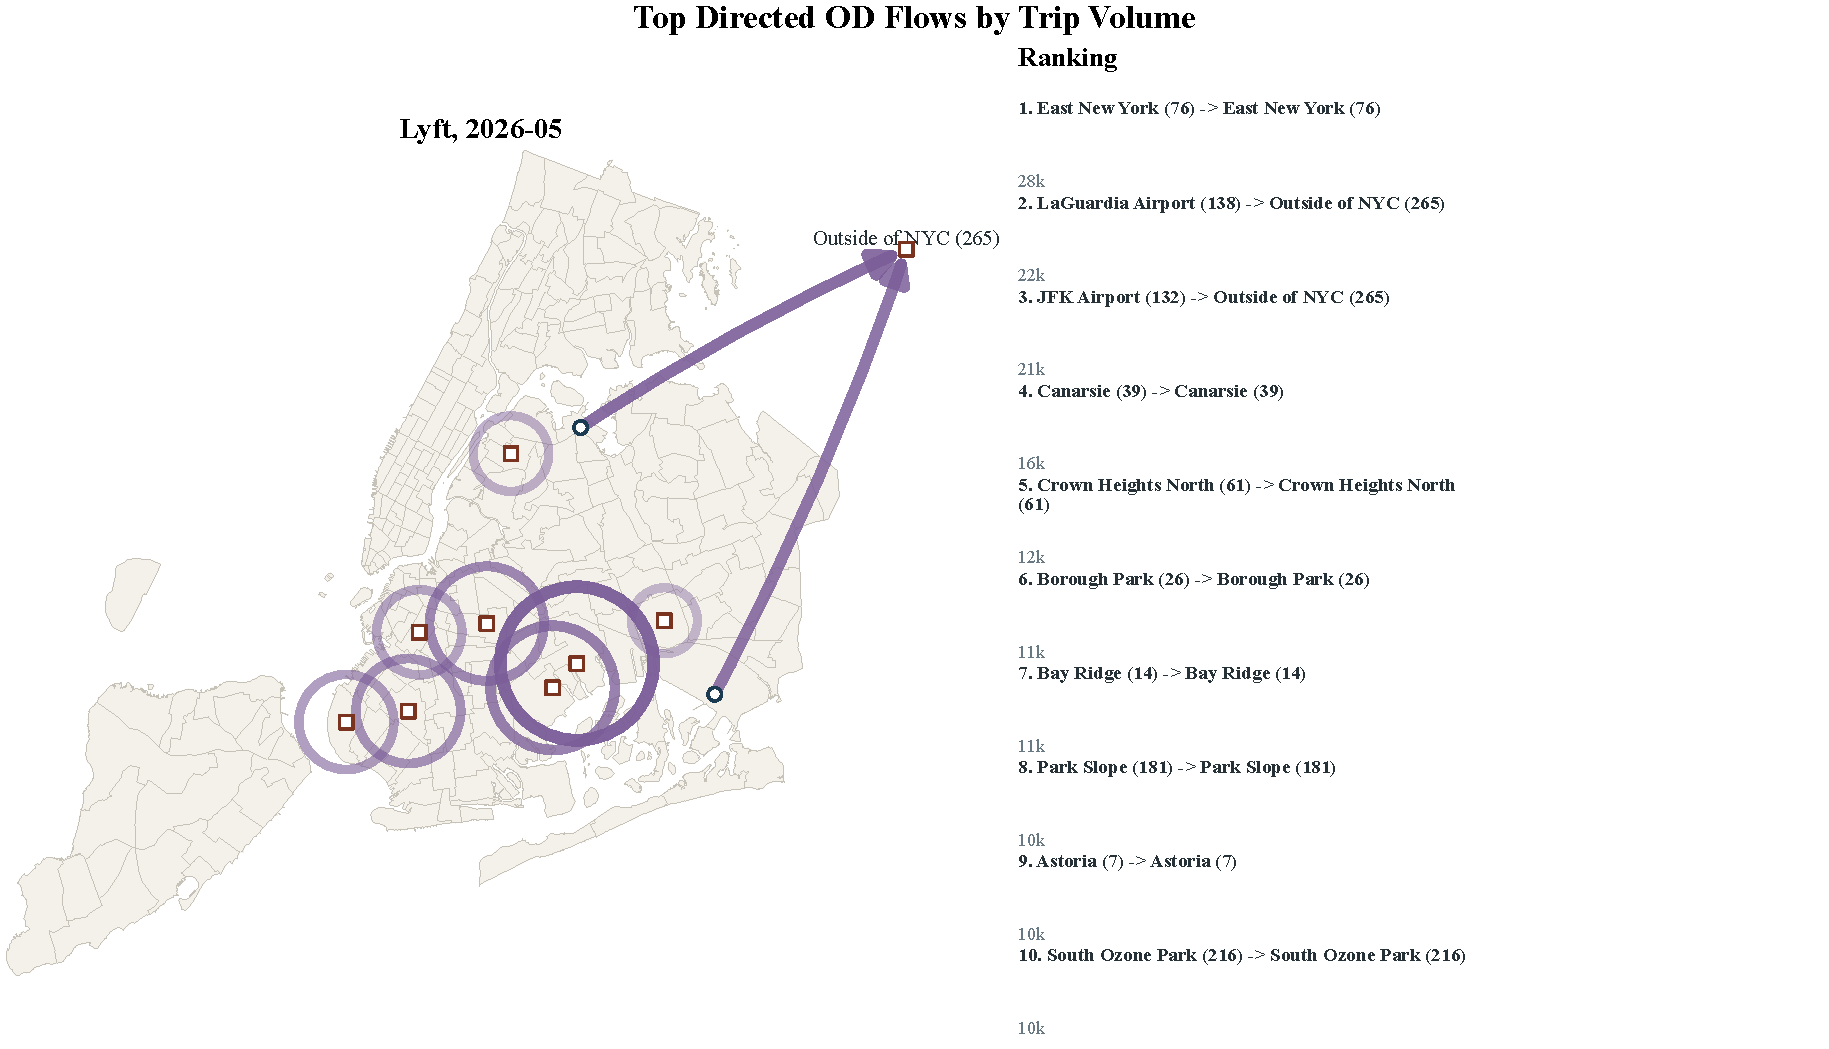
\includegraphics[height=.265\textheight,width=.98\linewidth,keepaspectratio]{04_Results/report_figures/appendix/task2_od_volume_2026-05_lyft.pdf}
\captionof{figure}{Top ten OD flows by trip volume, 2026-05. Panels from top to bottom: Yellow Taxi, Uber, and Lyft.}
\end{center}
\clearpage

\begin{center}
\centering
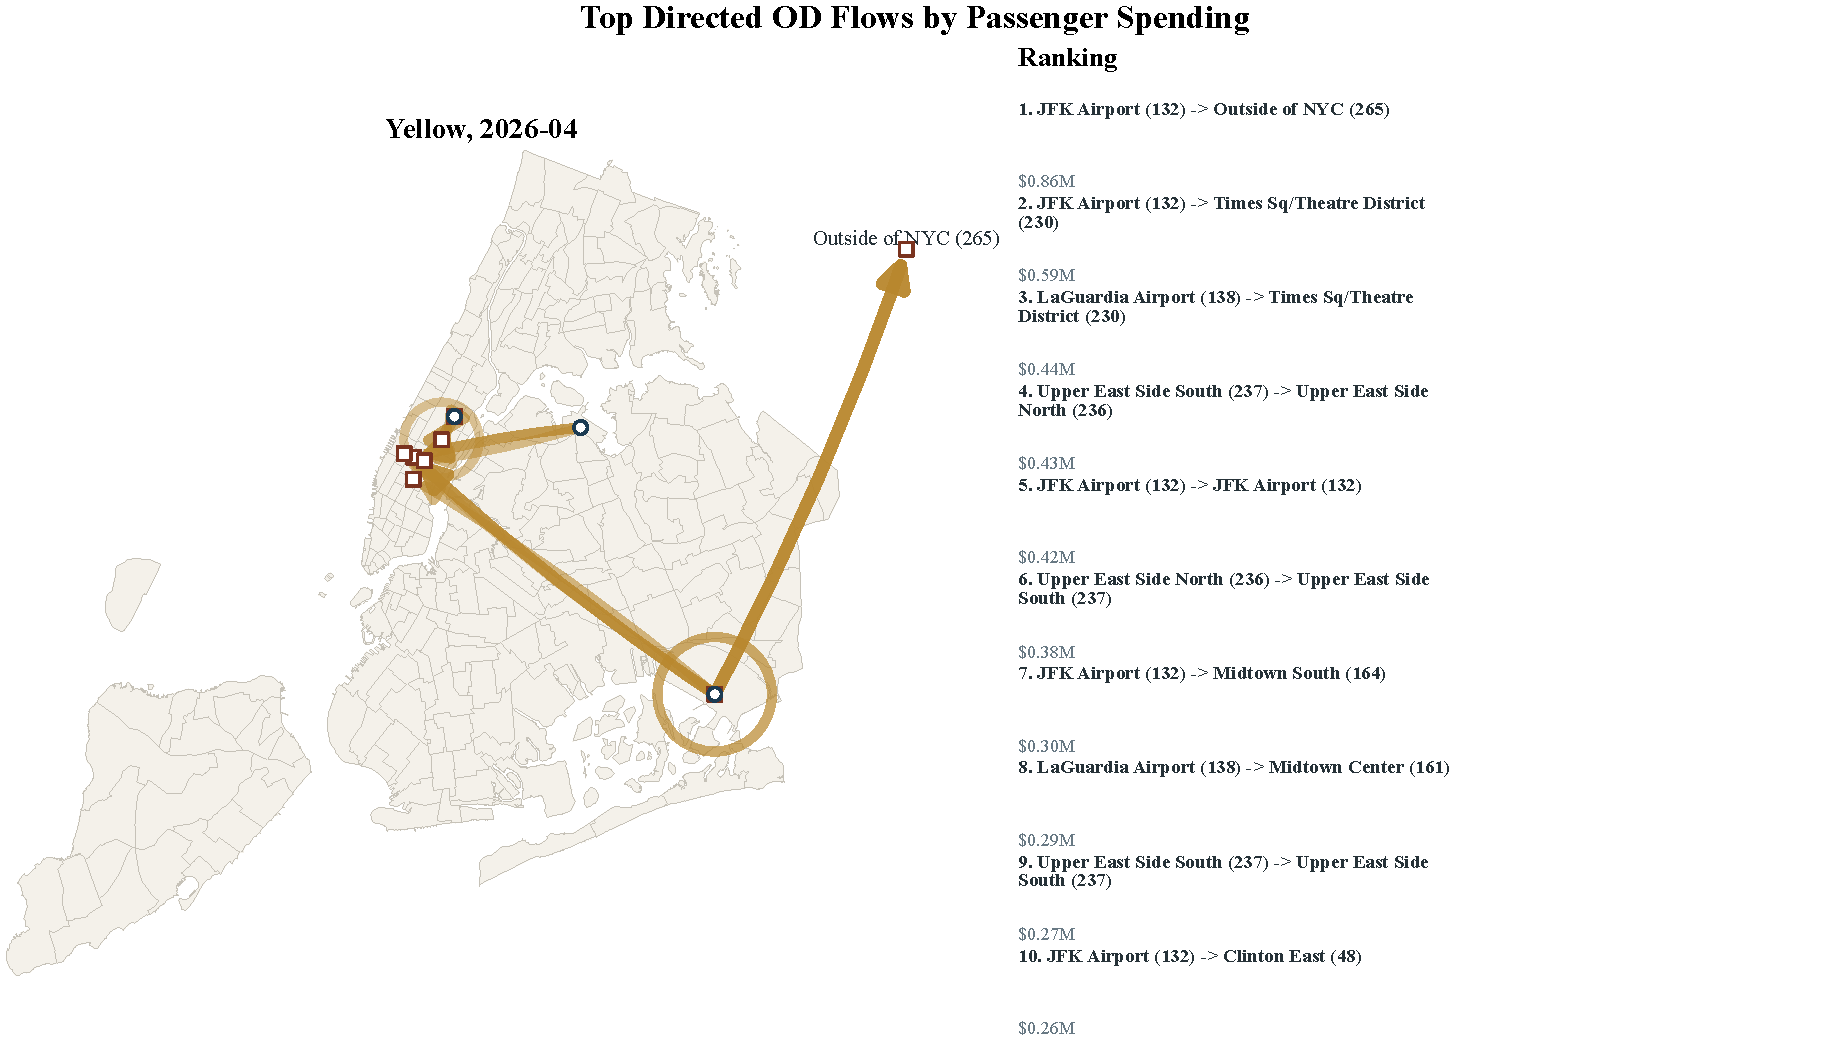
\includegraphics[height=.265\textheight,width=.98\linewidth,keepaspectratio]{04_Results/report_figures/appendix/task2_od_spending_2026-04_yellow.pdf}\par\vspace{0.2em}
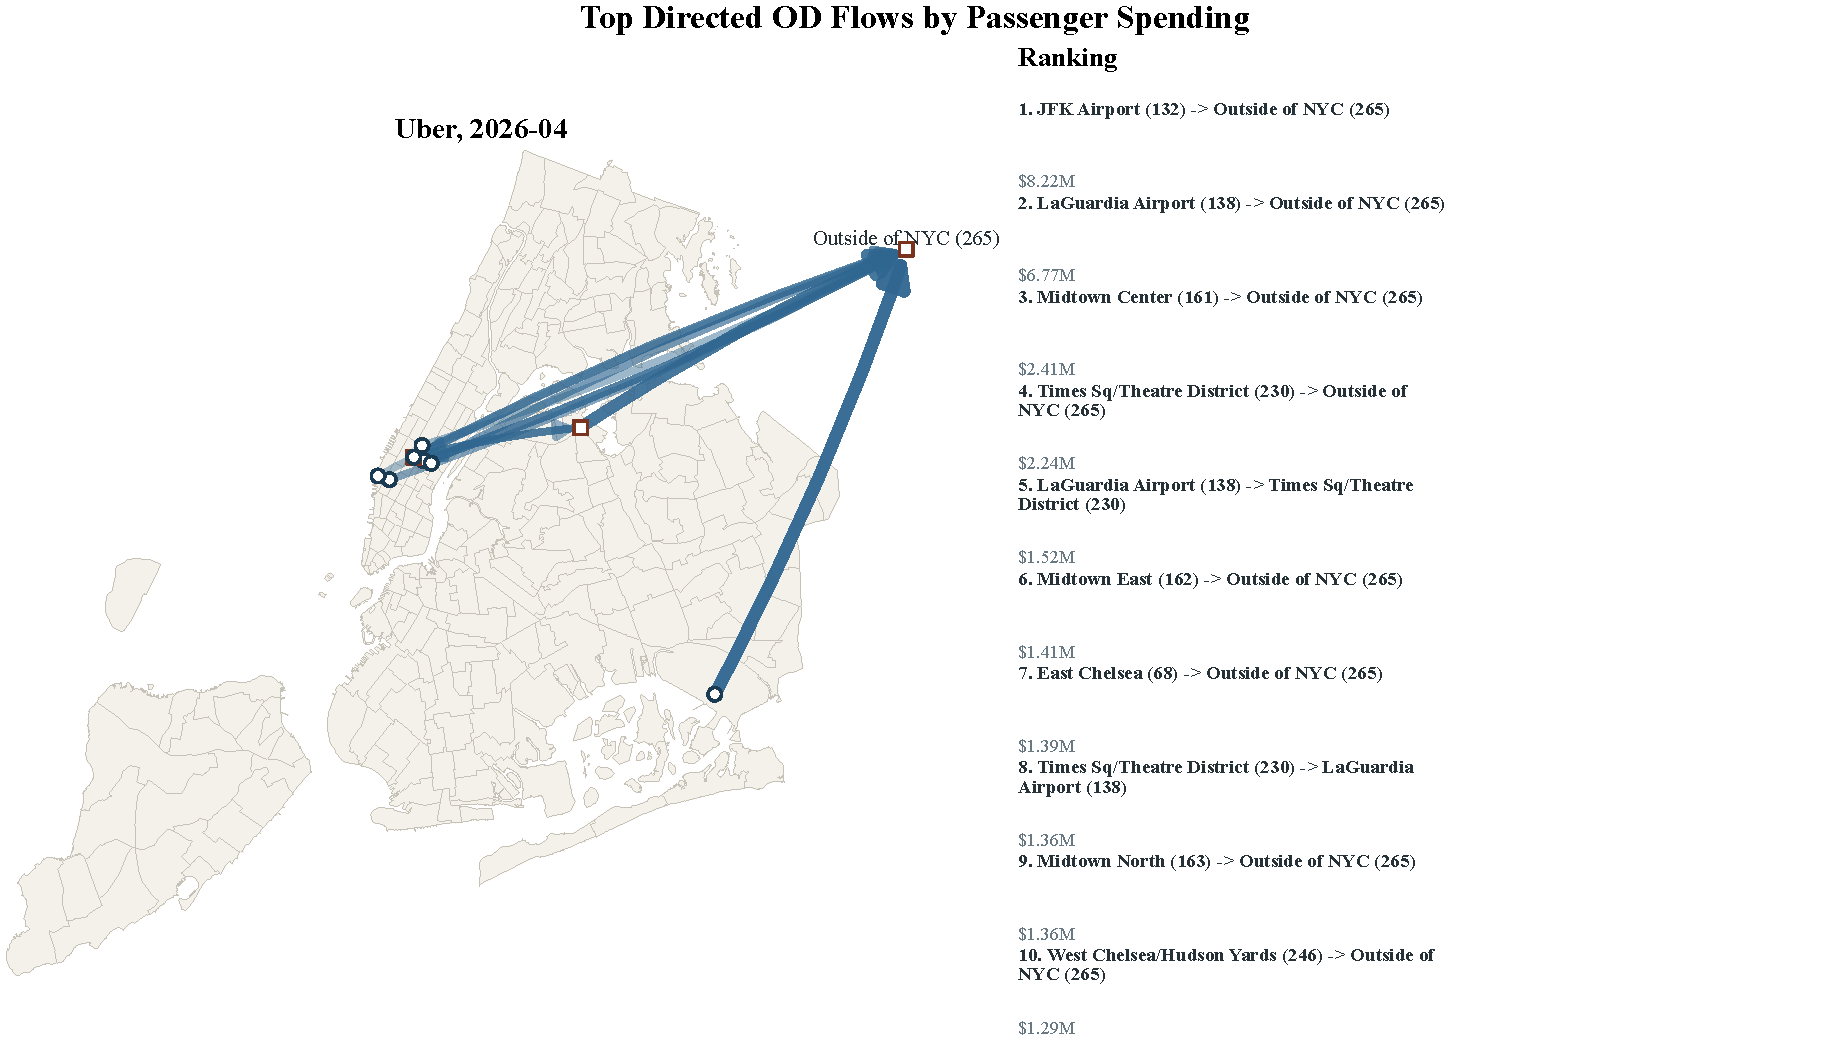
\includegraphics[height=.265\textheight,width=.98\linewidth,keepaspectratio]{04_Results/report_figures/appendix/task2_od_spending_2026-04_uber.pdf}\par\vspace{0.2em}
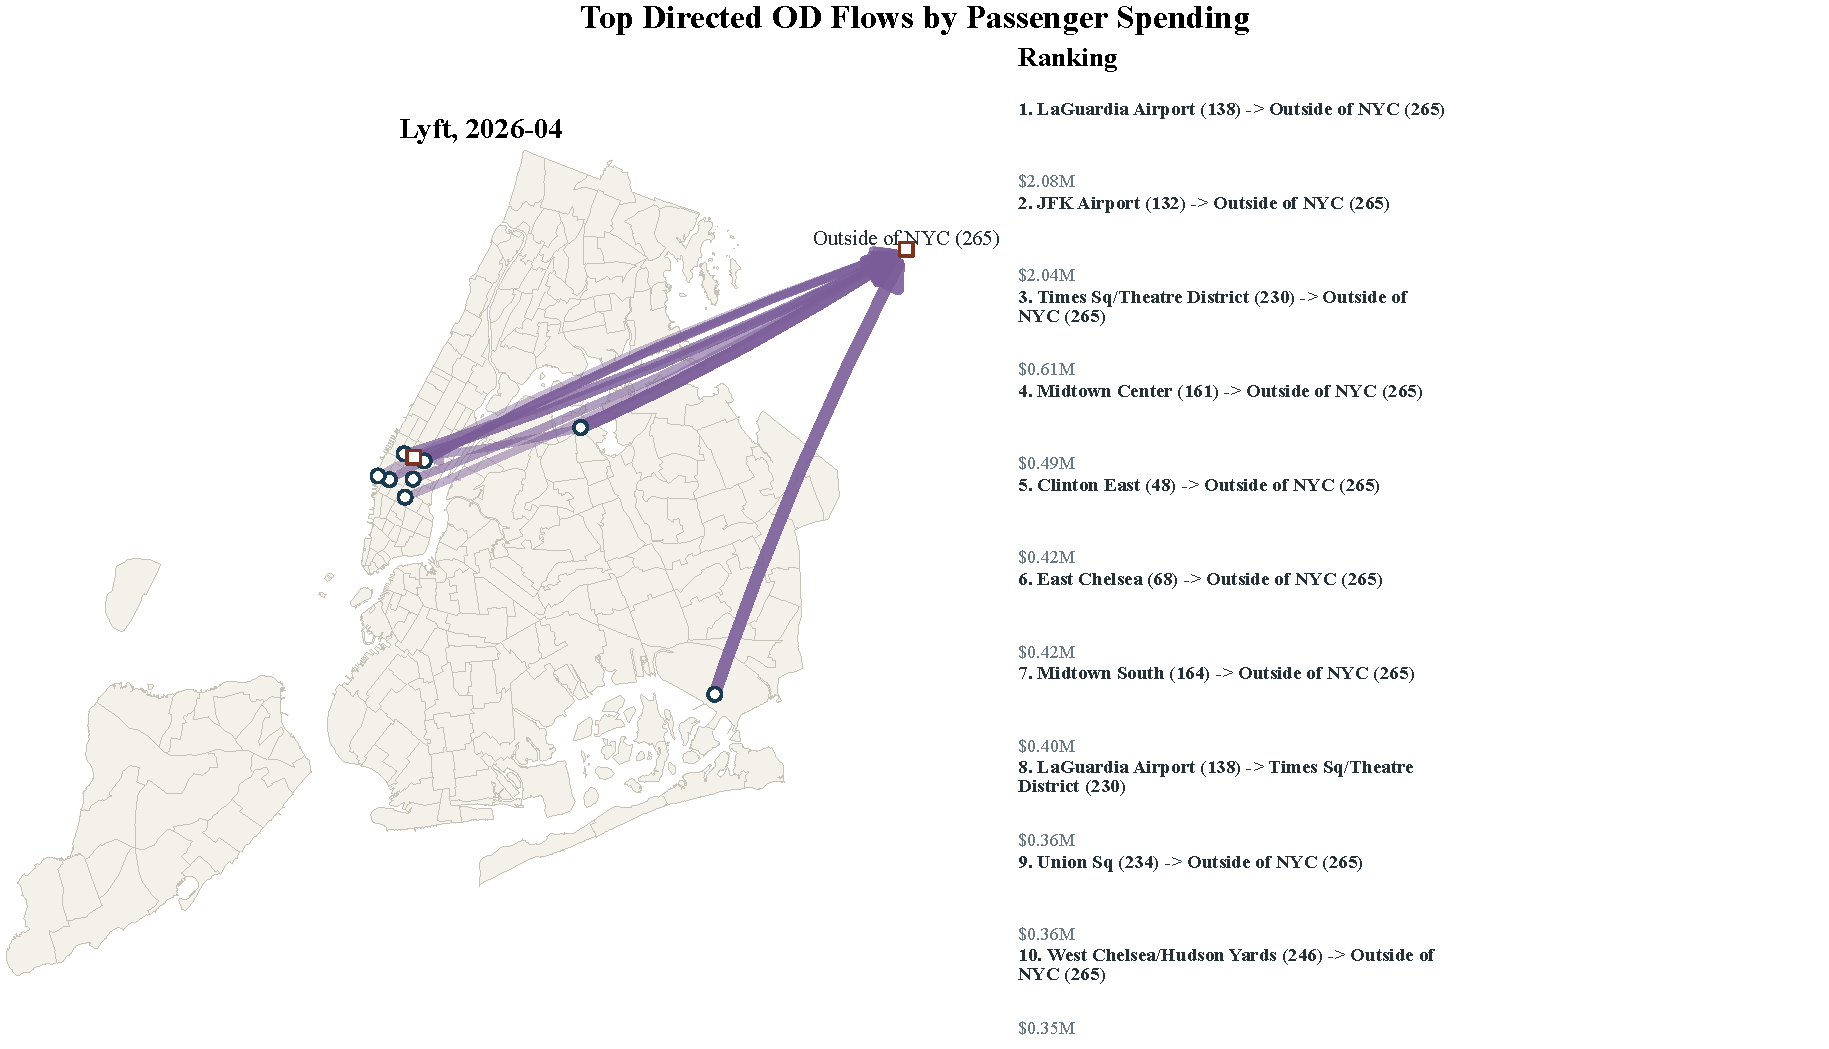
\includegraphics[height=.265\textheight,width=.98\linewidth,keepaspectratio]{04_Results/report_figures/appendix/task2_od_spending_2026-04_lyft.pdf}
\captionof{figure}{Top ten OD flows by aggregate passenger spending, 2026-04. Panels from top to bottom: Yellow Taxi, Uber, and Lyft.}
\end{center}
\clearpage

\begin{center}
\centering
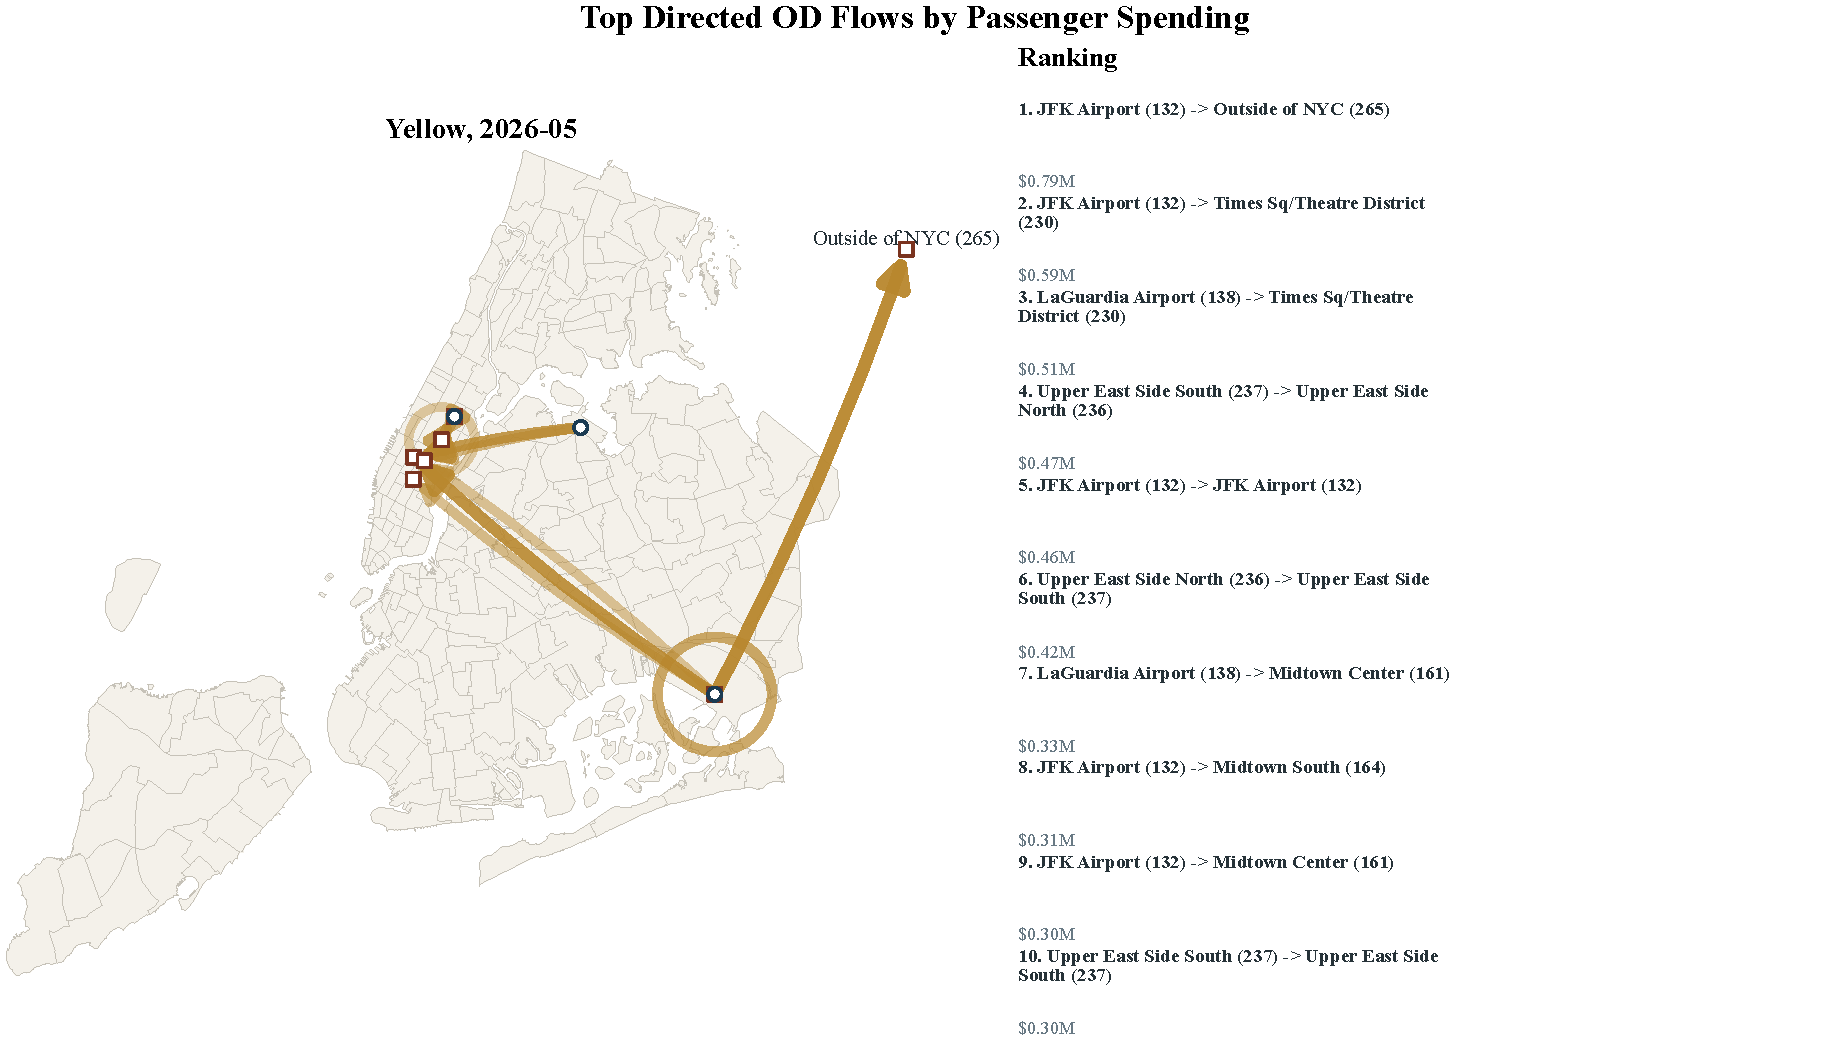
\includegraphics[height=.265\textheight,width=.98\linewidth,keepaspectratio]{04_Results/report_figures/appendix/task2_od_spending_2026-05_yellow.pdf}\par\vspace{0.2em}
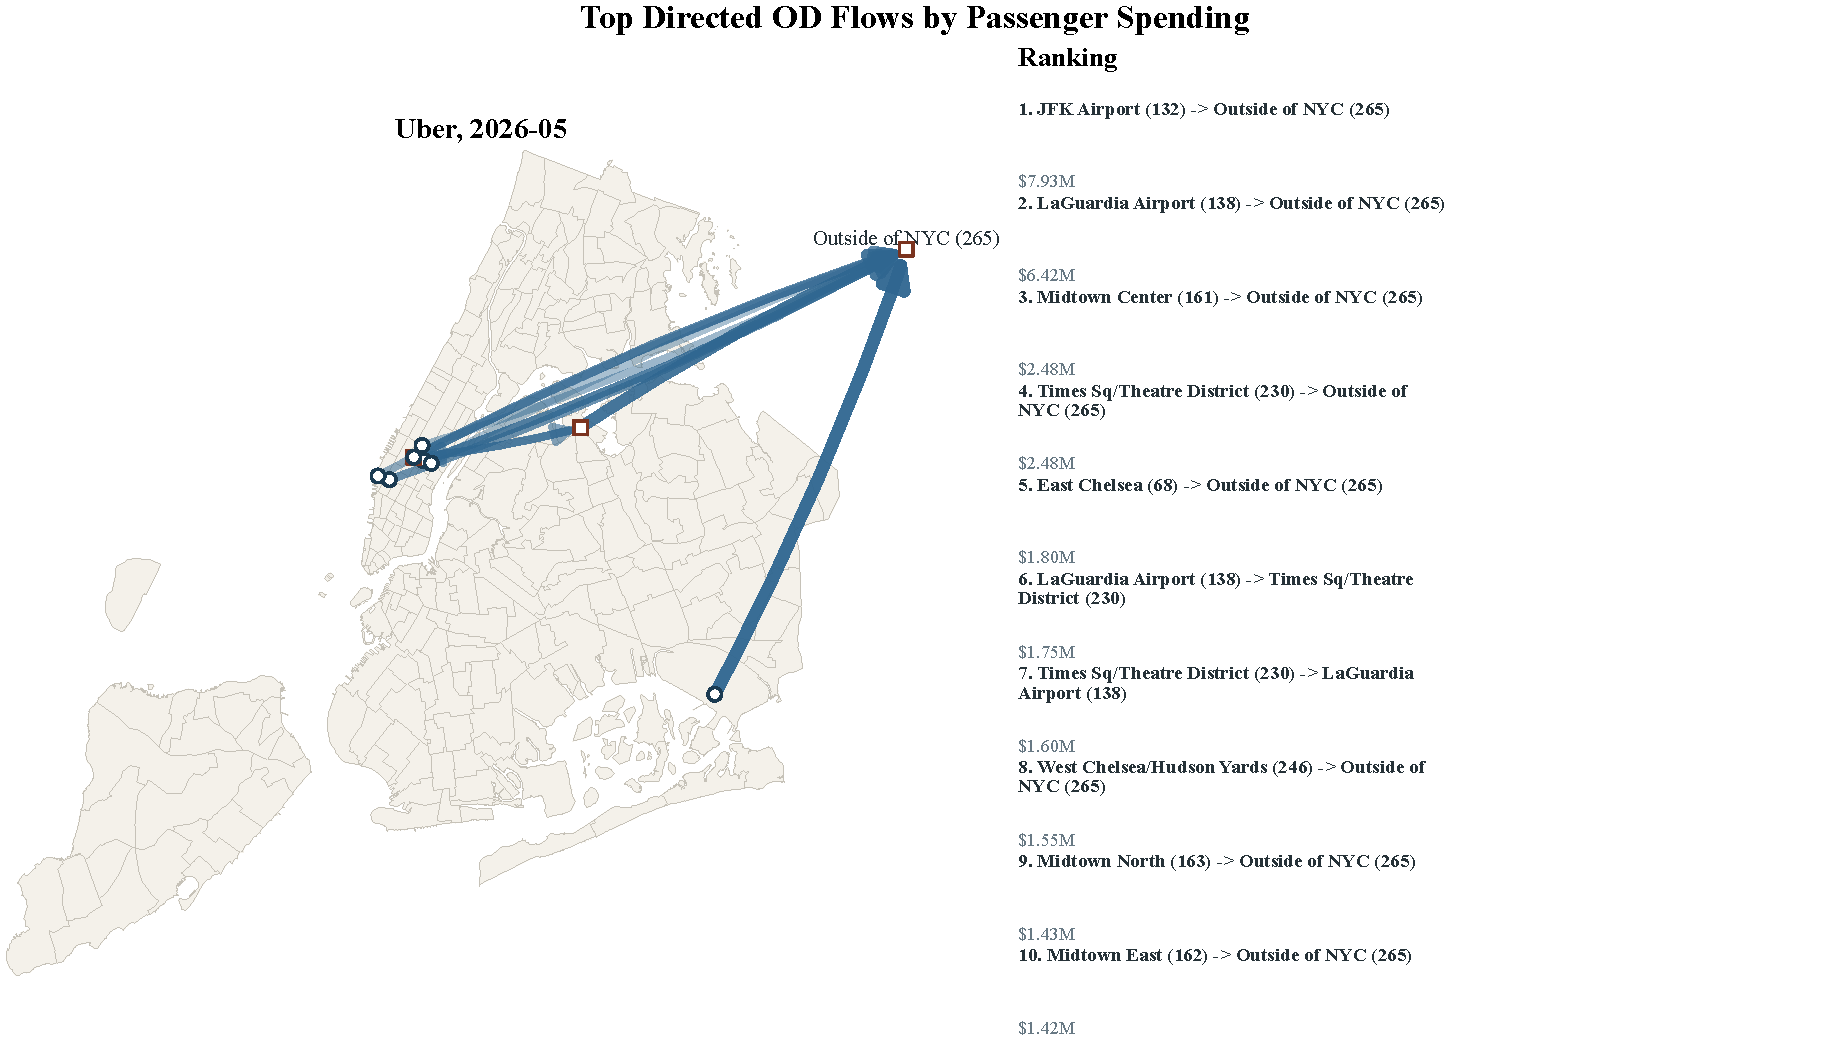
\includegraphics[height=.265\textheight,width=.98\linewidth,keepaspectratio]{04_Results/report_figures/appendix/task2_od_spending_2026-05_uber.pdf}\par\vspace{0.2em}
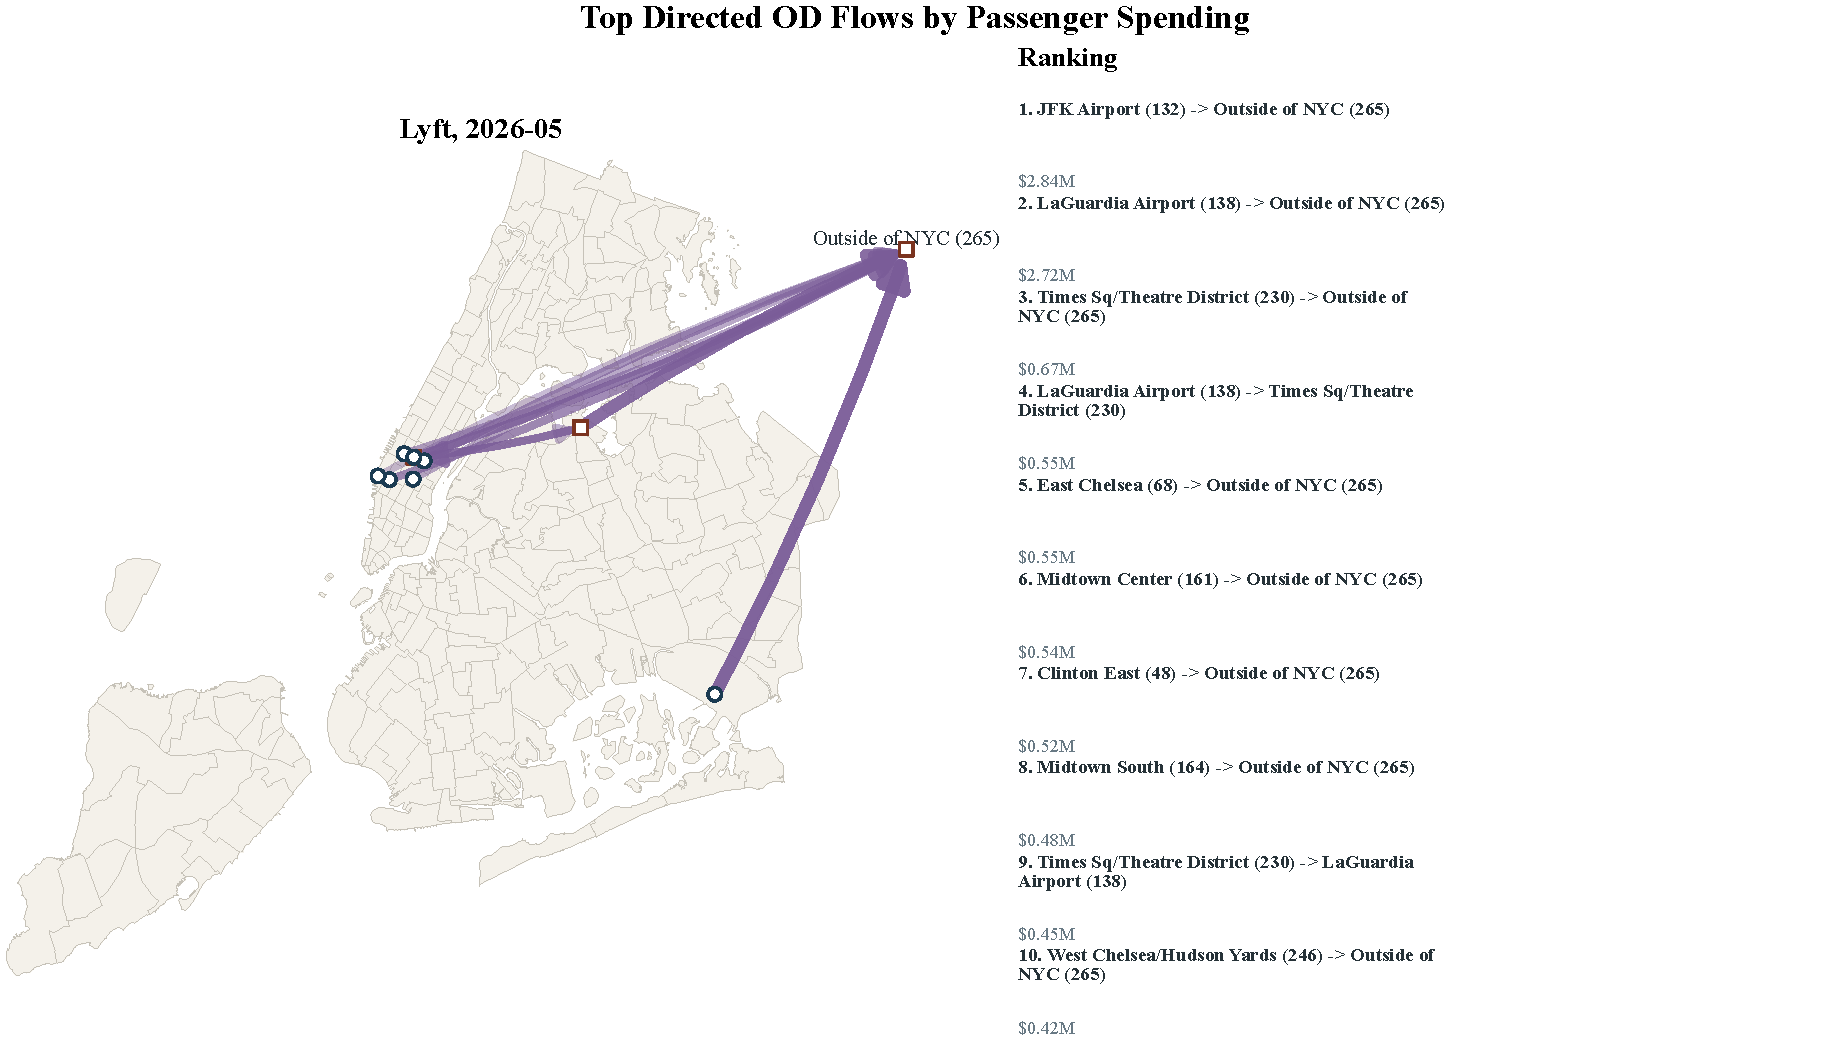
\includegraphics[height=.265\textheight,width=.98\linewidth,keepaspectratio]{04_Results/report_figures/appendix/task2_od_spending_2026-05_lyft.pdf}
\captionof{figure}{Top ten OD flows by aggregate passenger spending, 2026-05. Panels from top to bottom: Yellow Taxi, Uber, and Lyft.}
\end{center}
\clearpage

\subsection{Zone-level reported ride-pooling metrics}
Each panel reports pickup-zone request, match, and success metrics. Gray zones do not meet the required denominator threshold.

\begin{center}
\centering
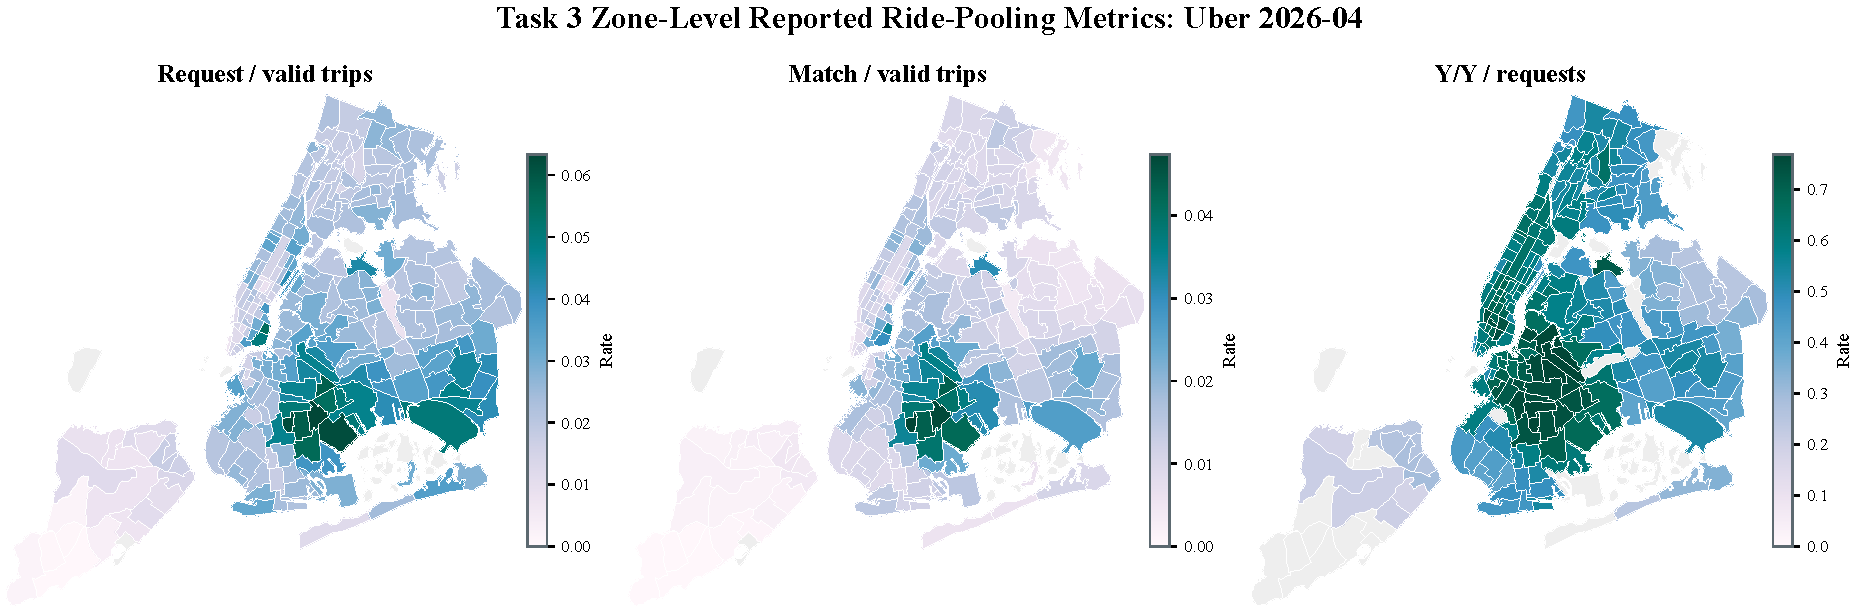
\includegraphics[height=.375\textheight,width=.98\linewidth,keepaspectratio]{04_Results/report_figures/appendix/task3_zone_metrics_2026-04_uber.pdf}\par\vspace{0.3em}
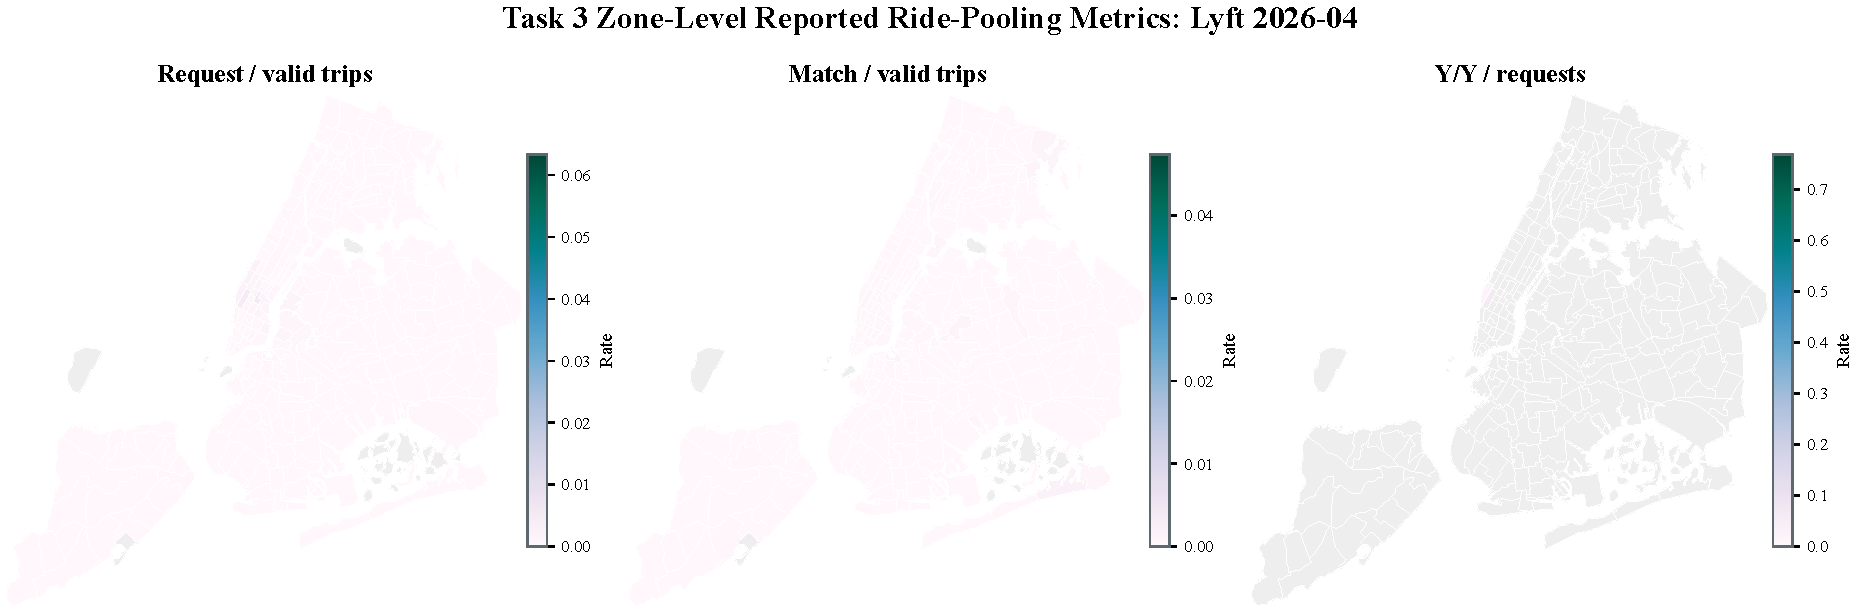
\includegraphics[height=.375\textheight,width=.98\linewidth,keepaspectratio]{04_Results/report_figures/appendix/task3_zone_metrics_2026-04_lyft.pdf}
\captionof{figure}{Zone-level reported ride-pooling metrics in 2026-04. Panels from top to bottom: Uber and Lyft. Gray zones have insufficient sample.}
\end{center}
\clearpage

\begin{center}
\centering
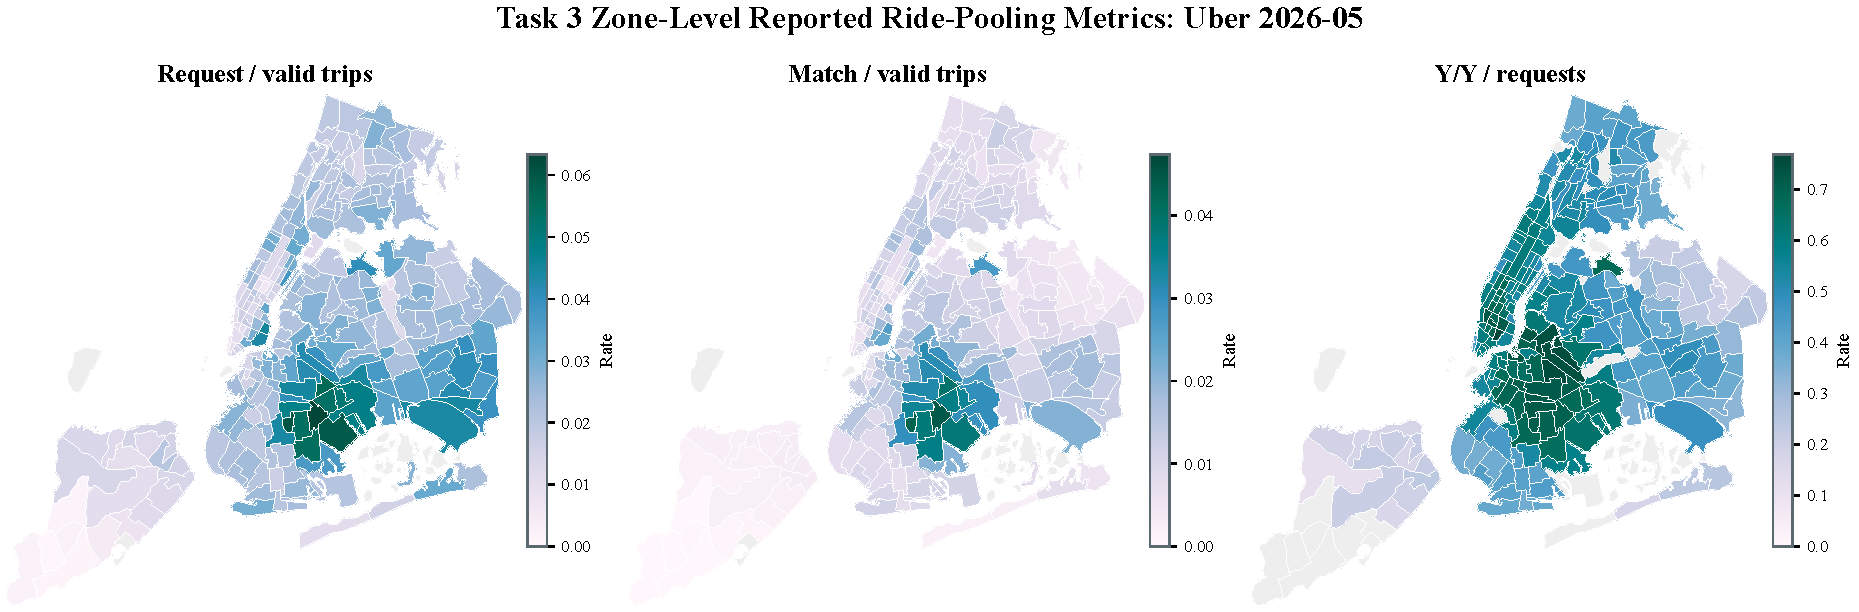
\includegraphics[height=.375\textheight,width=.98\linewidth,keepaspectratio]{04_Results/report_figures/appendix/task3_zone_metrics_2026-05_uber.pdf}\par\vspace{0.3em}
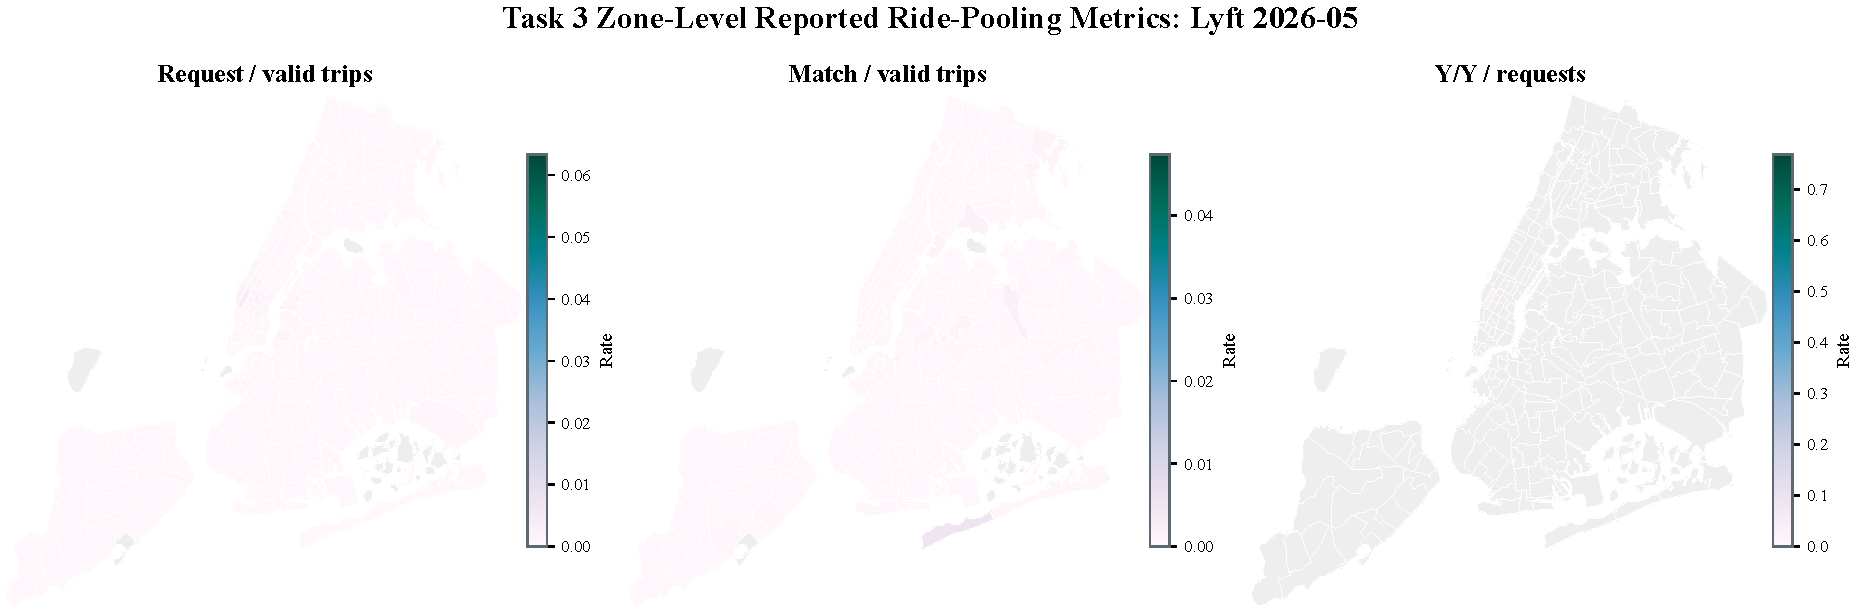
\includegraphics[height=.375\textheight,width=.98\linewidth,keepaspectratio]{04_Results/report_figures/appendix/task3_zone_metrics_2026-05_lyft.pdf}
\captionof{figure}{Zone-level reported ride-pooling metrics in 2026-05. Panels from top to bottom: Uber and Lyft. Gray zones have insufficient sample.}
\end{center}
\clearpage

\subsection{Spatial travel-time differences and reference coverage}
These maps show where supported Uber comparisons are available and how the observed mean travel-time difference varies by pickup zone.

\begin{center}
\centering
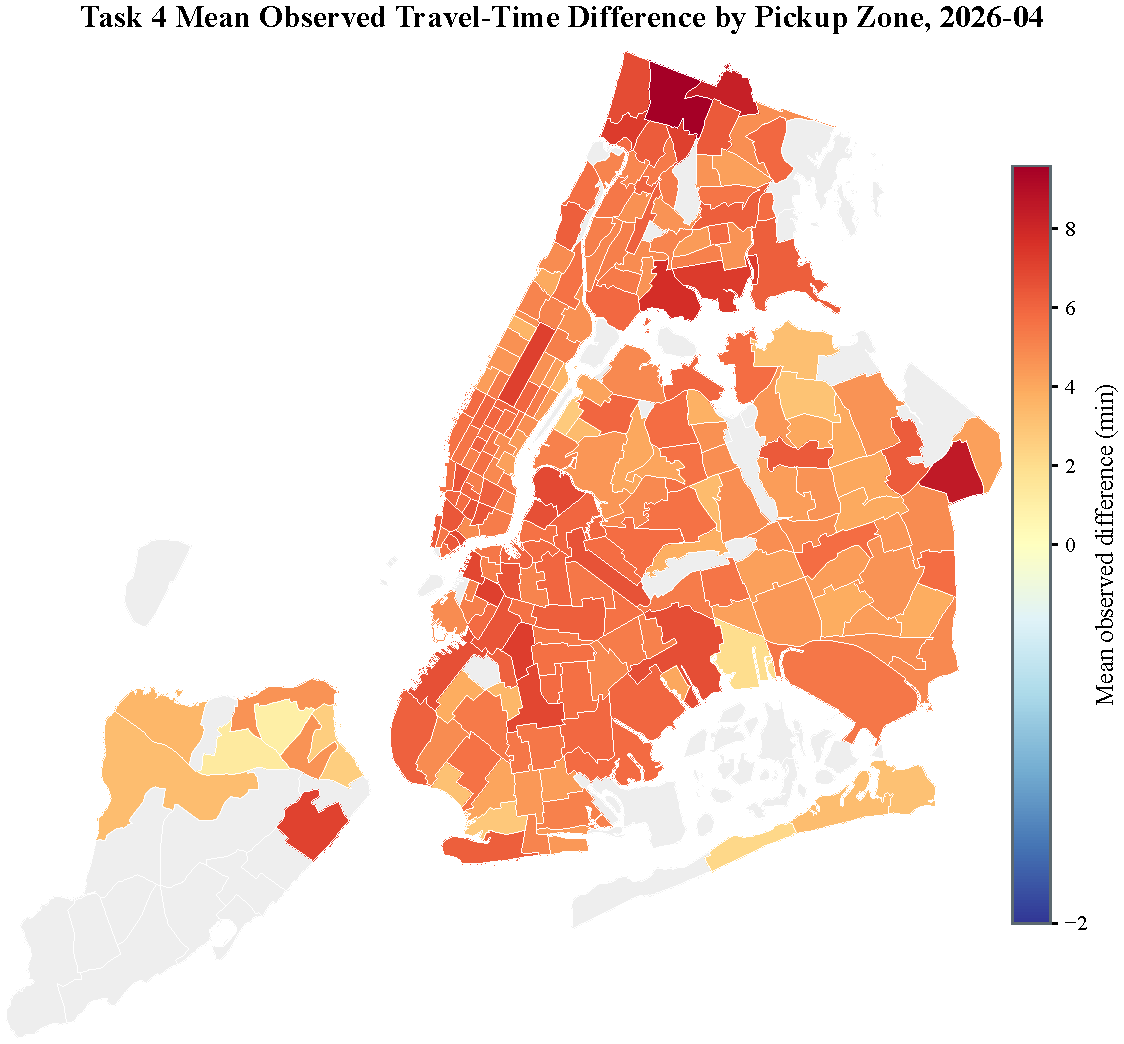
\includegraphics[height=.265\textheight,width=.98\linewidth,keepaspectratio]{04_Results/report_figures/appendix/task4_zone_mean_difference_2026-04.pdf}\par\vspace{0.2em}
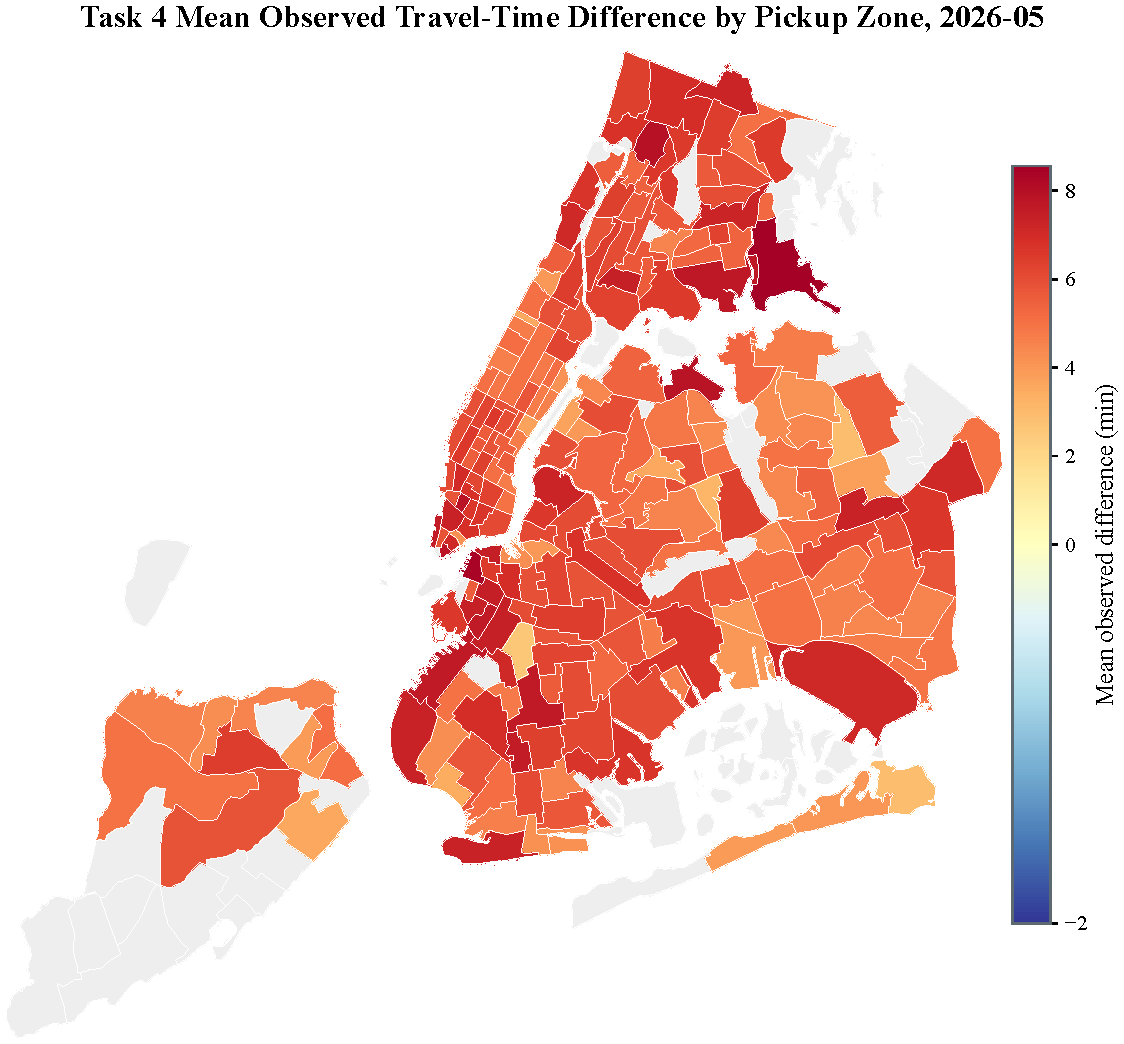
\includegraphics[height=.265\textheight,width=.98\linewidth,keepaspectratio]{04_Results/report_figures/appendix/task4_zone_mean_difference_2026-05.pdf}\par\vspace{0.2em}
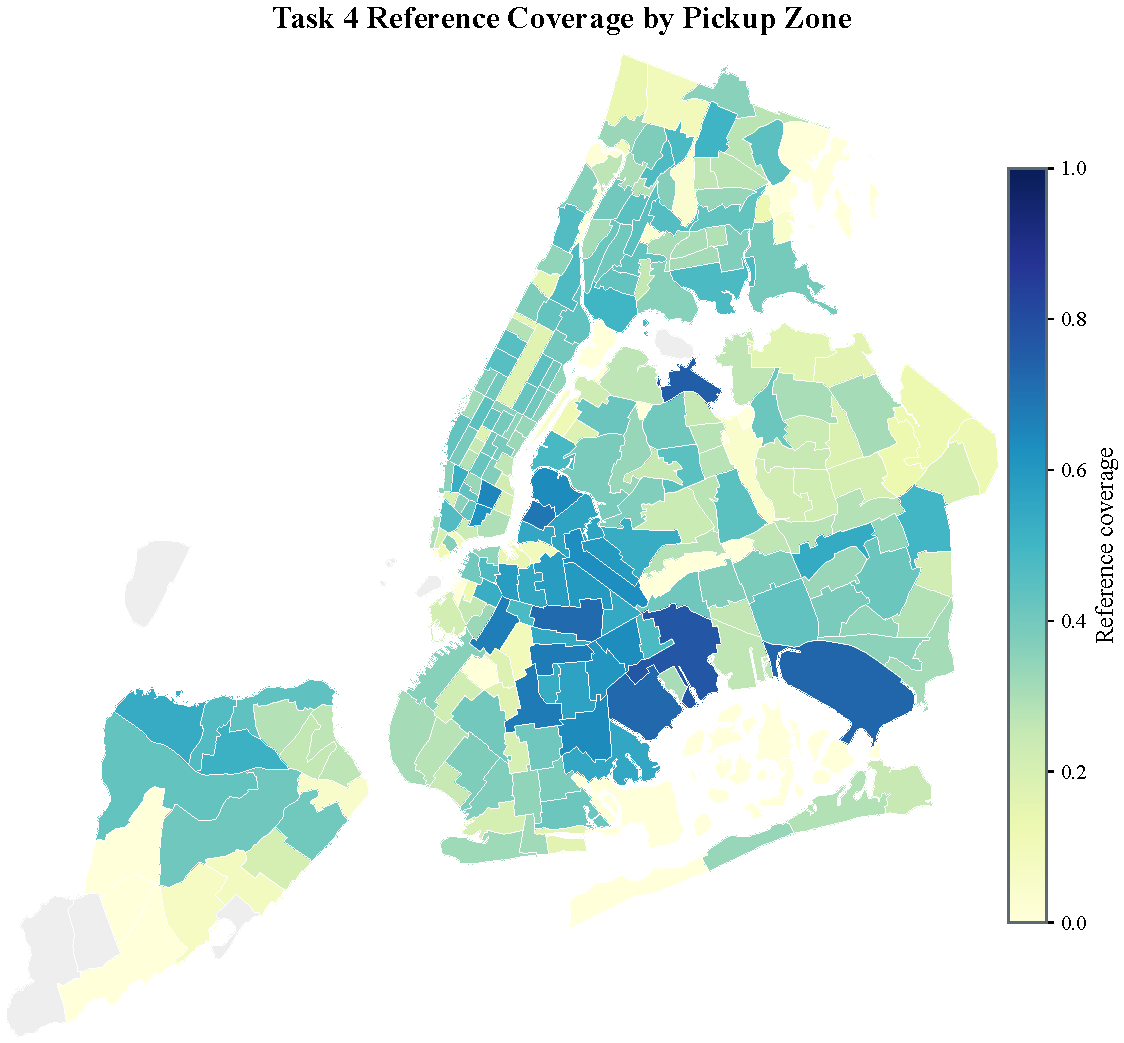
\includegraphics[height=.265\textheight,width=.98\linewidth,keepaspectratio]{04_Results/report_figures/appendix/task4_zone_reference_coverage.pdf}
\captionof{figure}{Spatial travel-time comparison diagnostics for Uber shared trips. Panels from top to bottom: April mean difference, May mean difference, and reference coverage.}
\end{center}

\endgroup
